\documentclass[10pt,twocolumn,letterpaper]{article}

\usepackage{cvpr}
\usepackage{times}
\usepackage{epsfig}
\usepackage{graphicx}
\usepackage{amsmath}
\usepackage{amssymb}
\usepackage{mathtools}

\DeclarePairedDelimiter\abs{\lvert}{\rvert}%

% Include other packages here, before hyperref.

% If you comment hyperref and then uncomment it, you should delete
% egpaper.aux before re-running latex.  (Or just hit 'q' on the first latex
% run, let it finish, and you should be clear).
\usepackage[breaklinks=true,bookmarks=false]{hyperref}

\cvprfinalcopy % *** Uncomment this line for the final submission

\def\cvprPaperID{****} % *** Enter the  Paper ID here
\def\httilde{\mbox{\tt\raisebox{-.5ex}{\symbol{126}}}}

% Pages are numbered in submission mode, and unnumbered in camera-ready
\setcounter{page}{4321}
\begin{document}

%%%%%%%%% TITLE
\title{EE3-23: Coursework for Introduction to Machine Learning}

\author{Douglas Brion\\
Imperial College London\\
CID: 01052925\\
{\tt\small db1415@ic.ac.uk}
}

\maketitle
%\thispagestyle{empty}


%%%%%%%%% BODY TEXT
\section{Introduction}

This report examines different approaches to predicting wine quality using the Wine Quality~\cite{WineQuality} dataset. This is a large dataset containing 4898 samples of white wines and 1599 of red. Throughout this report wine quality is examined using regression, attempting to predict the quality of a wine from various input parameters. Multiple learning methods are implemented, discussed and compared in order to obtain a predictor with the smallest test error possible.

%-------------------------------------------------------------------------
\section{Data Preparation}
Both red and white wine datasets were available and it was decided to combine both into a single dataset consisting of 6497 samples in order to learn how to predict the quality of either a red or white wine. 

The data provided in the now combined dataset was not normalised, therefore each attribute was normalised with respect to it's mean and standard deviation. Outliers over a threshold of $Thres = 5$ from each attribute were then removed to reduce noise in the dataset for training. This altered data was output to 
\verb+winequality-fixed.csv+.

\begin{figure}[h]
	\begin{center}
		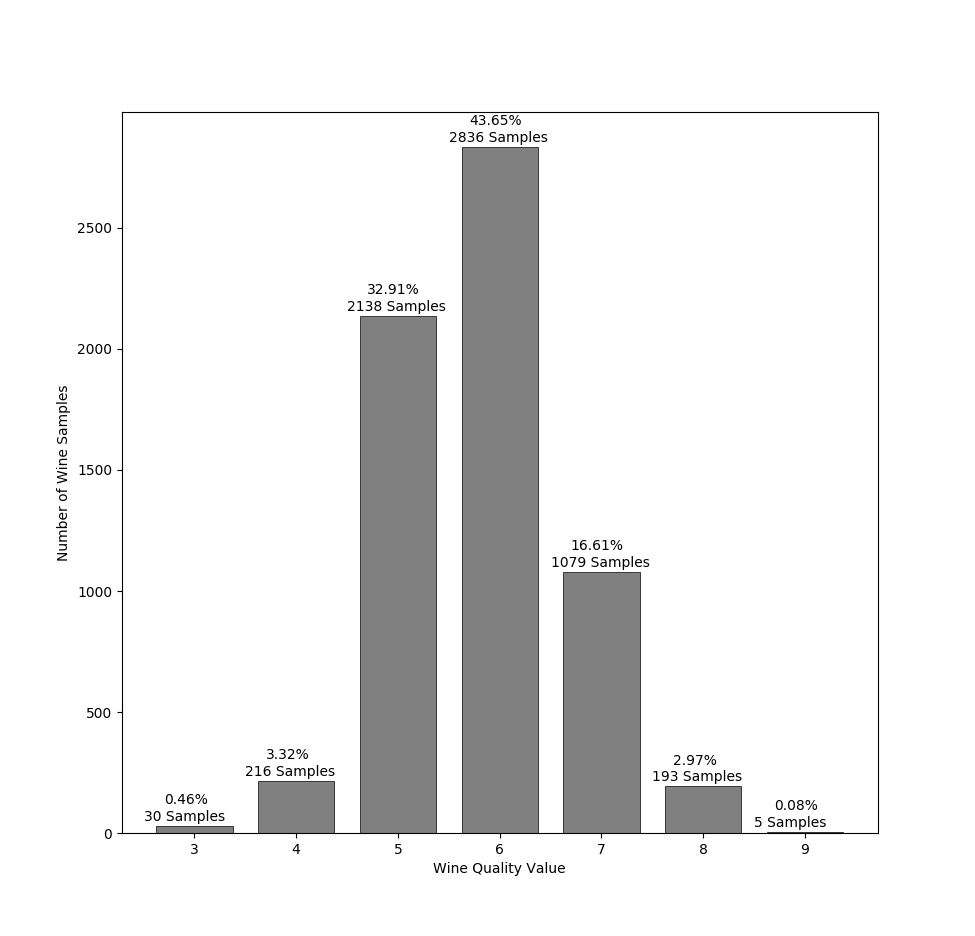
\includegraphics[width=0.9\linewidth]{samples.png}
	\end{center}
	\caption{The histogram for both white wine and red wine qualities.}
	\label{fig:long}
	\label{fig:onecol}
\end{figure}


\begin{table}[h]
	\begin{center}
		\begin{tabular}{|l|c|c|c|c|}
			\hline
			Attributes & Mean & Std & Min & Max \\
			\hline
			fixed acidity & 7.22 & 1.30 & 3.80 & 15.90 \\
			volatile acidity & 0.34 & 0.16 & 0.08 & 1.58 \\
			citric acid & 0.32 & 0.15 & 0.00 & 1.66 \\
			residual sugar & 5.44 & 4.76 & 0.60 & 65.80 \\
			chlorides & 0.06 & 0.04 & 0.01 & 0.61 \\
			free sulfur dioxide & 30.53 & 17.75 & 1.00 & 289.00 \\
			total sulfur dioxide & 115.74 & 56.52 & 6.00 & 440.00 \\
			density & 0.99 & 0.00 & 0.98 & 1.04 \\
			pH & 3.22 & 0.16 & 2.72 & 4.01 \\
			sulphates & 0.53 & 0.15 & 0.22 & 2.00 \\
			alcohol & 10.49 & 1.19 & 8.00 & 14.90 \\ 
			\hline
		\end{tabular}
	\end{center}
	\caption{The attribute statistics before normalisation and removal of outliers.}
\end{table}

\begin{table}[h]
	\begin{center}
		\begin{tabular}{|l|c|c|c|c|}
			\hline
			Attributes & Mean & Std & Min & Max \\
			\hline
			fixed acidity & -0.012 & 0.965 & -2.635 & 4.848 \\
			volatile acidity & -0.005 & 0.984 & -1.577 & 4.800 \\
			citric acid & -0.002 & 0.990 & -2.193 & 4.689 \\
			residual sugar & -0.004 & 0.983 & -1.018 & 4.331 \\
			chlorides & -0.049 & 0.740 & -1.343 & 4.966 \\
			free sulfur dioxide & -0.008 & 0.968 & -1.664 & 4.957 \\
			total sulfur dioxide & -0.001 & 0.998 & -1.942 & 4.437 \\
			density & -0.004 & 0.979 & -2.530 & 2.999 \\
			pH & 0.000 & 1.000 & -3.101 & 4.923 \\
			sulphates & -0.017 & 0.936 & -2.092 & 4.898 \\
			alcohol & 0.000 & 1.000 & -2.089 & 3.696 \\ 
			\hline
		\end{tabular}
	\end{center}
	\caption{The attribute statistics after normalisation and removal of outliers.}
\end{table}

\subsection{Learning approach}

For consistency all the different regressions performances of each model with varying parameters will be measured using the same error metric, mean absolute deviation. 

\begin{equation}
\frac{1}{n} \sum_{i = 1}^{n} \abs{x_i - m(X)}
\end{equation}

This shall be used on the test error of each of the models for comparison as each model will required a different training error.

\section{Learning Models}
Papers, excluding the references section,
must be no longer than requested pages in length. The references section
will not be included in the page count, and there is no limit on the
length of the references section. For example, a paper of four pages
with two pages of references would have a total length of 10 pages.

\subsection{Linear Regression}
Overlength papers will simply not be reviewed.  This includes papers
where the margins and formatting are deemed to have been significantly
altered from those laid down by this style guide.  Note that this
\LaTeX\ guide already sets figure captions and references in a smaller font.
The reason such papers will not be reviewed is that there is no provision for
supervised revisions of manuscripts.  

%-------------------------------------------------------------------------
\subsection{The ruler}
The \LaTeX\ style defines a printed ruler which should be present in the
version submitted for review.  The ruler is provided in order that
reviewers may comment on particular lines in the paper without
circumlocution.  If you are preparing a document using a non-\LaTeX\
document preparation system, please arrange for an equivalent ruler to
appear on the final output pages.  The presence or absence of the ruler
should not change the appearance of any other content on the page.  The
camera ready copy should not contain a ruler. (\LaTeX\ users may uncomment
the command in the document preamble.)  Reviewers:
note that the ruler measurements do not align well with lines in the paper
--- this turns out to be very difficult to do well when the paper contains
many figures and equations, and, when done, looks ugly.  Just use fractional
references (e.g.\ this line is $095.5$), although in most cases one would
expect that the approximate location will be adequate.

\subsection{Mathematics}

Please number all of your sections and displayed equations.  It is
important for readers to be able to refer to any particular equation.  Just
because you didn't refer to it in the text doesn't mean some future reader
might not need to refer to it.  It is cumbersome to have to use
circumlocutions like ``the equation second from the top of page 3 column
1''.  (Note that the ruler will not be present in the final copy, so is not
an alternative to equation numbers).  All authors will benefit from reading
Mermin's description of how to write mathematics:
\url{http://www.pamitc.org/documents/mermin.pdf}.




\begin{figure}[t]
\begin{center}
\fbox{\rule{0pt}{2in} \rule{0.9\linewidth}{0pt}}
   %\includegraphics[width=0.8\linewidth]{egfigure.eps}
\end{center}
   \caption{Example of caption.  It is set in Roman so that mathematics
   (always set in Roman: $B \sin A = A \sin B$) may be included without an
   ugly clash.}
\label{fig:long}
\label{fig:onecol}
\end{figure}

\subsection{Miscellaneous}

\noindent
Compare the following:\\
\begin{tabular}{ll}
 \verb'$conf_a$' &  $conf_a$ \\
 \verb'$\mathit{conf}_a$' & $\mathit{conf}_a$
\end{tabular}\\
See The \TeX book, p165.

The space after \eg, meaning ``for example'', should not be a
sentence-ending space. So \eg is correct, {\em e.g.} is not.  The provided
\verb'\eg' macro takes care of this.

When citing a multi-author paper, you may save space by using ``et alia'',
shortened to ``\etal'' (not ``{\em et.\ al.}'' as ``{\em et}'' is a complete word.)
However, use it only when there are three or more authors.  Thus, the
following is correct: ``
   Frobnication has been trendy lately.
   It was introduced by Alpher~\cite{Alpher02}, and subsequently developed by
   Alpher and Fotheringham-Smythe~\cite{Alpher03}, and Alpher \etal~\cite{Alpher04}.''

This is incorrect: ``... subsequently developed by Alpher \etal~\cite{Alpher03} ...''
because reference~\cite{Alpher03} has just two authors.  If you use the
\verb'\etal' macro provided, then you need not worry about double periods
when used at the end of a sentence as in Alpher \etal.

For this citation style, keep multiple citations in numerical (not
chronological) order, so prefer \cite{Alpher03,Alpher02,Authors14} to
\cite{Alpher02,Alpher03,Authors14}.


\begin{figure*}
\begin{center}
\fbox{\rule{0pt}{2in} \rule{.9\linewidth}{0pt}}
\end{center}
   \caption{Example of a short caption, which should be centered.}
\label{fig:short}
\end{figure*}

%------------------------------------------------------------------------
\section{Formatting your paper}

All text must be in a two-column format. The total allowable width of the
text area is $6\frac78$ inches (17.5 cm) wide by $8\frac78$ inches (22.54
cm) high. Columns are to be $3\frac14$ inches (8.25 cm) wide, with a
$\frac{5}{16}$ inch (0.8 cm) space between them. The main title (on the
first page) should begin 1.0 inch (2.54 cm) from the top edge of the
page. The second and following pages should begin 1.0 inch (2.54 cm) from
the top edge. On all pages, the bottom margin should be 1-1/8 inches (2.86
cm) from the bottom edge of the page for $8.5 \times 11$-inch paper; for A4
paper, approximately 1-5/8 inches (4.13 cm) from the bottom edge of the
page.

%-------------------------------------------------------------------------
\subsection{Margins and page numbering}

All printed material, including text, illustrations, and charts, must be kept
within a print area 6-7/8 inches (17.5 cm) wide by 8-7/8 inches (22.54 cm)
high.
Page numbers should be in footer with page numbers, centered and .75
inches from the bottom of the page and make it start at the correct page
number rather than the 4321 in the example.  To do this fine the line (around
line 23)
\begin{verbatim}
%\ifcvprfinal\pagestyle{empty}\fi
\setcounter{page}{4321}
\end{verbatim}
where the number 4321 is your assigned starting page.

Make sure the first page is numbered by commenting out the first page being
empty on line 46
\begin{verbatim}
%\thispagestyle{empty}
\end{verbatim}


%-------------------------------------------------------------------------
\subsection{Type-style and fonts}

Wherever Times is specified, Times Roman may also be used. If neither is
available on your word processor, please use the font closest in
appearance to Times to which you have access.

MAIN TITLE. Center the title 1-3/8 inches (3.49 cm) from the top edge of
the first page. The title should be in Times 14-point, boldface type.
Capitalize the first letter of nouns, pronouns, verbs, adjectives, and
adverbs; do not capitalize articles, coordinate conjunctions, or
prepositions (unless the title begins with such a word). Leave two blank
lines after the title.

AUTHOR NAME(s) and AFFILIATION(s) are to be centered beneath the title
and printed in Times 12-point, non-boldface type. This information is to
be followed by two blank lines.

The ABSTRACT and MAIN TEXT are to be in a two-column format.

MAIN TEXT. Type main text in 10-point Times, single-spaced. Do NOT use
double-spacing. All paragraphs should be indented 1 pica (approx. 1/6
inch or 0.422 cm). Make sure your text is fully justified---that is,
flush left and flush right. Please do not place any additional blank
lines between paragraphs.

Figure and table captions should be 9-point Roman type as in
Figures~\ref{fig:onecol} and~\ref{fig:short}.  Short captions should be centred.

\noindent Callouts should be 9-point Helvetica, non-boldface type.
Initially capitalize only the first word of section titles and first-,
second-, and third-order headings.

FIRST-ORDER HEADINGS. (For example, {\large \bf 1. Introduction})
should be Times 12-point boldface, initially capitalized, flush left,
with one blank line before, and one blank line after.

SECOND-ORDER HEADINGS. (For example, { \bf 1.1. Database elements})
should be Times 11-point boldface, initially capitalized, flush left,
with one blank line before, and one after. If you require a third-order
heading (we discourage it), use 10-point Times, boldface, initially
capitalized, flush left, preceded by one blank line, followed by a period
and your text on the same line.

%-------------------------------------------------------------------------
\subsection{Footnotes}

Please use footnotes\footnote {This is what a footnote looks like.  It
often distracts the reader from the main flow of the argument.} sparingly.
Indeed, try to avoid footnotes altogether and include necessary peripheral
observations in
the text (within parentheses, if you prefer, as in this sentence).  If you
wish to use a footnote, place it at the bottom of the column on the page on
which it is referenced. Use Times 8-point type, single-spaced.


%-------------------------------------------------------------------------
\subsection{References}

List and number all bibliographical references in 9-point Times,
single-spaced, at the end of your paper. When referenced in the text,
enclose the citation number in square brackets, for
example~\cite{Authors14}.  Where appropriate, include the name(s) of
editors of referenced books.


%-------------------------------------------------------------------------
\subsection{Illustrations, graphs, and photographs}

All graphics should be centered.  Please ensure that any point you wish to
make is resolvable in a printed copy of the paper.  Resize fonts in figures
to match the font in the body text, and choose line widths which render
effectively in print.  Many readers (and reviewers), even of an electronic
copy, will choose to print your paper in order to read it.  You cannot
insist that they do otherwise, and therefore must not assume that they can
zoom in to see tiny details on a graphic.

When placing figures in \LaTeX, it's almost always best to use
\verb+\includegraphics+, and to specify the  figure width as a multiple of
the line width as in the example below
{\small\begin{verbatim}
   \usepackage[dvips]{graphicx} ...
   \includegraphics[width=0.8\linewidth]
                   {myfile.eps}
\end{verbatim}
}





{\small
\bibliographystyle{ieee}
\bibliography{egbib}
}

\end{document}
